% !TeX root = main.tex

\section{Intégration à Géofoncier et évaluation des résultats}
\label{sec:integration}

Ce chapitre présente la dernière phase du traitement : le versement sur Géofoncier. Il décrit d'abord en détail comment l'appel à l'API est géré techniquement, puis expose le mode de traitement, avant de suivre un dossier réel de bout en bout et de conclure sur une évaluation du système.

\subsection{Fonctionnement du versement}

Le chapitre~\ref{sec:analyse_metier} a présenté la structure de l'API REST Géofoncier et le format des données qu'elle attend. Cette section décrit comment le script \texttt{geofoncier\_api.py} met en pratique ces échanges, du jeton d'authentification jusqu'à l'upload du document source.

Les identifiants du cabinet (login et mot de passe Géofoncier) sont stockés dans un fichier \texttt{.env} local, qui n'est jamais partagé ni versionné. L'authentification repose sur une requête \texttt{GET /token} avec une en-tête \texttt{Authorization: Basic base64(login:password)}.

Au démarrage de l'application, la fonction \texttt{get\_valid\_token()} décode la date d'expiration inscrite dans le jeton JWT (champ \texttt{exp}) et calcule le temps restant. Si l'expiration est à moins de 30 minutes, un nouveau jeton est demandé automatiquement. Ce mécanisme est entièrement transparent pour l'opérateur. La durée de validité réelle d'un jeton est de 10 heures.

En cas d'échec du renouvellement, l'ancienne valeur du jeton est conservée en mémoire et l'interface affiche un avertissement. Si aucun jeton valide n'est disponible au moment du versement, l'API retourne un \texttt{401 Unauthorized}, que l'interface traduit en message explicite.

Lorsque l'opérateur clique sur \enquote{Créer le dossier sur Géofoncier}, l'application construit le dictionnaire de données à partir de toutes les informations collectées lors des étapes précédentes. La fonction \texttt{create\_geofoncier\_dossier()} assemble ensuite le payload JSON avant l'envoi. Ce dictionnaire rassemble les identifiants Géofoncier du cabinet créateur (\texttt{enr\_cab\_createur}, par exemple \texttt{1987I004169}) et du cabinet détenteur (\texttt{enr\_cab\_detenteur}), la référence interne du dossier (\texttt{enr\_ref\_dossier}, limitée à 15 caractères), le code INSEE à 5 chiffres (\texttt{enr\_code\_insee}), ainsi que la date de l'opération au format ISO 8601 (\texttt{enr\_date\_dossier}). Il spécifie aussi le code d'opération (\texttt{op\_code}, comme \texttt{Em} pour une modification parcellaire ou \texttt{Eb} pour un bornage), la liste des parcelles cadastrales, les coordonnées Lambert-93 du marqueur sur la carte (\texttt{localisant}), le numéro DMPC formaté (\texttt{dmpc\_ref}) et le statut du dossier (\texttt{enr\_statut}).

Détail des éléments transmis dans ce dictionnaire :
\begin{itemize}
  \item Identifiants du cabinet : les champs \texttt{enr\_cab\_createur} et \texttt{enr\_cab\_detenteur} reçoivent le numéro d'inscription du cabinet à l'Ordre des Géomètres-Experts.
  \item Référence et commune : le champ \texttt{enr\_ref\_dossier} enregistre la référence interne (15 caractères maximum), \texttt{enr\_code\_insee} le code de la commune à 5 chiffres, et \texttt{enr\_date\_dossier} la date au format ISO.
  \item Type d'opération : le champ \texttt{op\_code} précise la nature de l'acte (\texttt{Em} pour division, \texttt{Eb} pour bornage), et \texttt{enr\_statut} indique le niveau de validation.
  \item Localisant géométrique : l'objet \texttt{localisant} contient une structure de point GeoJSON avec les coordonnées du marqueur calculées en Lambert-93 (EPSG:2154).
  \item Parcelles concernées : la liste \texttt{parcelles} rassemble les objets précisant la section cadastrale et le numéro de chaque parcelle modifiée.
\end{itemize}

Chaque champ fait l'objet d'un contrôle automatique avant la requête, comme expliqué lors de la fiabilisation au chapitre~\ref{sec:fiabilisation}. Si le code INSEE ou les coordonnées sont absents, le script bloque la préparation et alerte l'opérateur dans l'interface.

Avant l'envoi, le dictionnaire est converti en JSON. Les coordonnées spatiales en Lambert-93 sont arrondies à deux décimales (précision centimétrique). Les chaînes de caractères sont encodées en UTF-8 pour prévenir toute altération des caractères accentués lors du transit HTTP.

Le transfert des requêtes vers le serveur de Géofoncier s'appuie sur la bibliothèque \texttt{requests} avec une gestion des délais d'attente. Si le serveur de la plateforme met plus de 15 secondes à répondre (en période de forte charge), l'application effectue jusqu'à trois tentatives successives avec un délai d'attente avant de lever une exception et de proposer une sauvegarde locale temporaire à l'utilisateur.

Le marqueur positionné par l'opérateur sur la carte est en coordonnées géographiques WGS84 (latitude/longitude). L'API Géofoncier attend des coordonnées en Lambert-93 (système officiel français, EPSG:2154). La conversion est assurée par la fonction \texttt{latlon\_to\_lambert93()}, qui utilise la bibliothèque \texttt{pyproj} si elle est disponible, ou à défaut une formule intégrée.

La requête \texttt{POST /dossiersoge/dossiers/} est envoyée avec le payload JSON dans le corps et le jeton dans l'en-tête \texttt{Authorization}. L'appel est synchrone : l'interface affiche un spinner pendant l'envoi.

En cas de succès, l'API retourne un code \texttt{201 Created} et un objet JSON contenant le champ \texttt{id} du dossier créé. Ce champ est affiché directement dans l'interface et enregistré dans le CSV de travail.

L'API peut également rejeter le champ \texttt{dmpc\_ref} si le format du numéro de DA ne correspond pas à celui attendu côté serveur. Le script gère ce cas avec un mécanisme de repli : il détecte le code d'erreur \texttt{400} associé à ce champ, supprime \texttt{dmpc\_ref} du payload et relance la requête sans lui. Le dossier est ainsi créé même si la référence DMPC n'a pas pu être attachée.

Après la création réussie du dossier, une deuxième requête \texttt{POST /dossiersoge/documents/} est envoyée en \texttt{multipart/form-data} pour attacher le fichier PDF au dossier. Le type MIME est détecté automatiquement depuis l'extension du fichier (\texttt{.pdf}, \texttt{.tif}, \texttt{.jpg}, etc.). Si le fichier source est introuvable dans le dossier d'entrée, l'interface signale l'absence sans bloquer : le dossier est déjà créé sur Géofoncier.

Plusieurs situations peuvent provoquer un échec lors du versement. Le Tableau~\ref{tab:erreurs_api} liste les principaux cas identifiés et les réponses apportées par le système.


\begin{table}[H]
  \centering
  \caption{Principaux cas d'erreur lors du versement sur l'API Géofoncier.}
  \label{tab:erreurs_api}
  \small
  \begin{tabular}{p{3.5cm}p{3.5cm}p{5cm}}
    \toprule
    \textbf{Cause} & \textbf{Code HTTP} & \textbf{Réponse du système} \\
    \midrule
    Token expiré ou invalide & \texttt{401 Unauthorized} & Message d'erreur dans l'interface, invitation à relancer l'application. \\
    \addlinespace
    Code INSEE manquant ou invalide & \texttt{400 Bad Request} & Blocage du bouton de versement dès la saisie ; le champ est marqué en rouge. \\
    \addlinespace
    Champ \texttt{dmpc\_ref} refusé & \texttt{400 Bad Request} & Repli automatique : nouvelle tentative sans ce champ. \\
    \addlinespace
    Données manquantes (référence vide) & Bloqué côté client & Le bouton est désactivé tant que la référence dossier n'est pas renseignée. \\
    \addlinespace
    Perte réseau pendant l'envoi & Exception Python & Message d'erreur avec le détail du payload envoyé pour diagnostic. \\
    \bottomrule
  \end{tabular}
\end{table}

Dans tous les cas d'échec, l'interface affiche le message d'erreur retourné par l'API et propose un panneau dépliable avec le contenu exact du payload, pour permettre de diagnostiquer la cause sans avoir à consulter les logs.

\subsection{Sécurisation du versement et traçabilité des échanges}

La transmission de données foncières vers une plateforme nationale exige un niveau élevé de contrôle afin de prémunir le cabinet contre tout risque de publication erronée ou de mauvaise interprétation.

\textbf{Contrôle de doublons et vérification d'intégrité avant envoi.} Avant de déclencher l'appel REST vers l'API Géofoncier, l'application interroge le registre local de suivi pour vérifier si la référence du dossier ou le document source a déjà fait l'objet d'une publication réussie. Si un doublon potentiel est détecté, l'interface affiche un message de mise en garde et bloque l'envoi direct, demandant une confirmation explicite à l'opérateur. De plus, une empreinte numérique (hash SHA-256) du fichier PDF source est calculée au moment du chargement. Cette empreinte est conservée dans l'historique local pour garantir qu'aucune modification ultérieure du fichier n'intervienne sans que la traçabilité ne soit rompue.

\textbf{Protocoles de communication des identifiants.} Toutes les requêtes transmises à l'API Géofoncier s'effectuent exclusivement en HTTPS via TLS 1.3, ce qui garantit le chiffrement de bout en bout des échanges sur le réseau. Les jetons JWT d'authentification sont stockés temporairement en mémoire vive au cours de la session applicative et ne sont jamais enregistrés dans des fichiers de sous-produits ou de journaux d'événements. Cette séparation stricte protège les identifiants professionnels du cabinet contre toute extraction non autorisée.

\textbf{responsabilité déontologique.} En vertu des règles déontologiques régissant la profession de géomètre-expert, toute publication sur le portail Géofoncier engage la responsabilité du cabinet détenteur du fonds. Pour répondre à cette exigence, chaque action de versement donne lieu à la rédaction automatique d'un journal d'audit infalsifiable. Ce journal consigne l'identifiant de l'opérateur connecté, l'adresse IP de la station de travail, l'horodatage exact au format UTC, la référence du dossier, le code INSEE de la commune ainsi que le contenu intégral de la réponse HTTP renvoyée par le serveur distant. Ces données fournissent une preuve technique incontestable en cas de contrôle de conformité ou de recherche d'historique.

\subsection{Mode de traitement par lot : \texttt{export\_geofoncier.py}}

En complément de l'interface de validation, un script de service (\texttt{export\_geofoncier.py}) permet de traiter des lots de documents sans intervention manuelle document par document. Ce script est prévu pour être lancé en tâche de fond, en parallèle du traitement OCR.

Son fonctionnement repose sur une boucle infinie qui scanne le dossier \texttt{outputs/} toutes les 30 secondes. À chaque itération, le script liste tous les fichiers JSON produits par la chaîne d'extraction (nommés selon le schéma \texttt{*\_plan\_*.json}) qui n'ont pas encore été traités. Pour chacun, il appelle \texttt{create\_geofoncier\_dossier()} avec le JSON comme source de données, puis tente d'uploader le PDF associé depuis \texttt{inputs/}. Une fois le traitement terminé (avec succès ou échec définitif), le fichier JSON est déplacé dans le sous-dossier \texttt{outputs/archives\_publiees/} pour ne pas être retraité au prochain scan.

Ce mode est particulièrement adapté au traitement de fonds entiers : une boîte de documents scannés peut être injectée dans \texttt{inputs/}, l'extraction automatique tourne la nuit, et les dossiers sont versés sur Géofoncier au fur et à mesure que les JSON sont produits. La supervision humaine reste indirecte : l'opérateur consulte le registre de suivi le lendemain pour vérifier les résultats.

\textbf{Le registre de suivi.} Après chaque versement, le script enregistre une entrée dans deux fichiers stockés dans le dossier \texttt{suivi\_geofoncier/}. Le premier fichier, \texttt{suivi\_publications.json}, conserve l'historique complet des versements (horodatage, commune, code INSEE, géomètre, référence du dossier, identifiant Géofoncier, nom du document source et statut final). Le second, \texttt{suivi\_publications.csv}, propose un tableau équivalent trié par commune puis par date, directement exploitable sous Excel ou LibreOffice.

Ces fichiers constituent la trace locale du travail effectué. Ils permettent aux associés du cabinet de savoir exactement quels dossiers ont été versés, à quelle date et sous quel identifiant Géofoncier, sans avoir à interroger l'API ni à consulter le portail.

En cas de coupure de réseau ou de panne temporaire du serveur distant pendant l'exécution par lot, le script conserve les requêtes non abouties dans une file d'attente locale de réessai. Les fichiers JSON correspondants ne sont pas déplacés vers le sous-dossier d'archivage, mais restent en attente. Dès la reconnexion au réseau, le script reprend l'envoi de la file d'attente à partir du dernier point d'échec sans risquer de créer des doublons d'actes sur le serveur Géofoncier.


\subsection{Déroulement d'un cas d'étude : commune de Prades}

Cette section suit le traitement d'un dossier réel de bout en bout, depuis le document papier jusqu'à la pastille créée sur Géofoncier.

Le document traité est un DMPC numérisé, issu du fonds du cabinet, concernant la commune de Prades (code INSEE~: \texttt{07182}), section cadastrale A. Il s'agit d'un formulaire imprimé d'une page, complété à la main. Le fichier est fourni au programme sous forme de PDF, placé dans le dossier d'entrée.

Le script de classification analyse le fichier et le reconnaît comme un DMPC en quelques secondes, sur la base de sa structure. Le modèle VLM traite ensuite les onze zones d'intérêt découpées par YOLOv8 sur la page. L'extraction automatique identifie la commune de Prades avec un indice de confiance de 92\,\% (validé à 100\,\% dans le référentiel de l'Ardèche), la section cadastrale A à 95\,\%, ainsi que le numéro d'ordre 3854 à 70\,\% (la présence d'un chiffre parasite 4 étant provoquée par le coin d'un tampon en marge, rapidement relevé par le contrôle de cohérence). Le nom du géomètre est détecté par balayage textuel (80\,\%), et la nature de l'acte est déduite comme étant un bornage.

Le contrôle de cohérence en quatre couches retourne un statut conforme avec un score de 100\,\%. L'image annotée générée par le traitement est reproduite en Figure~\ref{fig:harrois_annote}.

\begin{figure}[H]
  \centering
  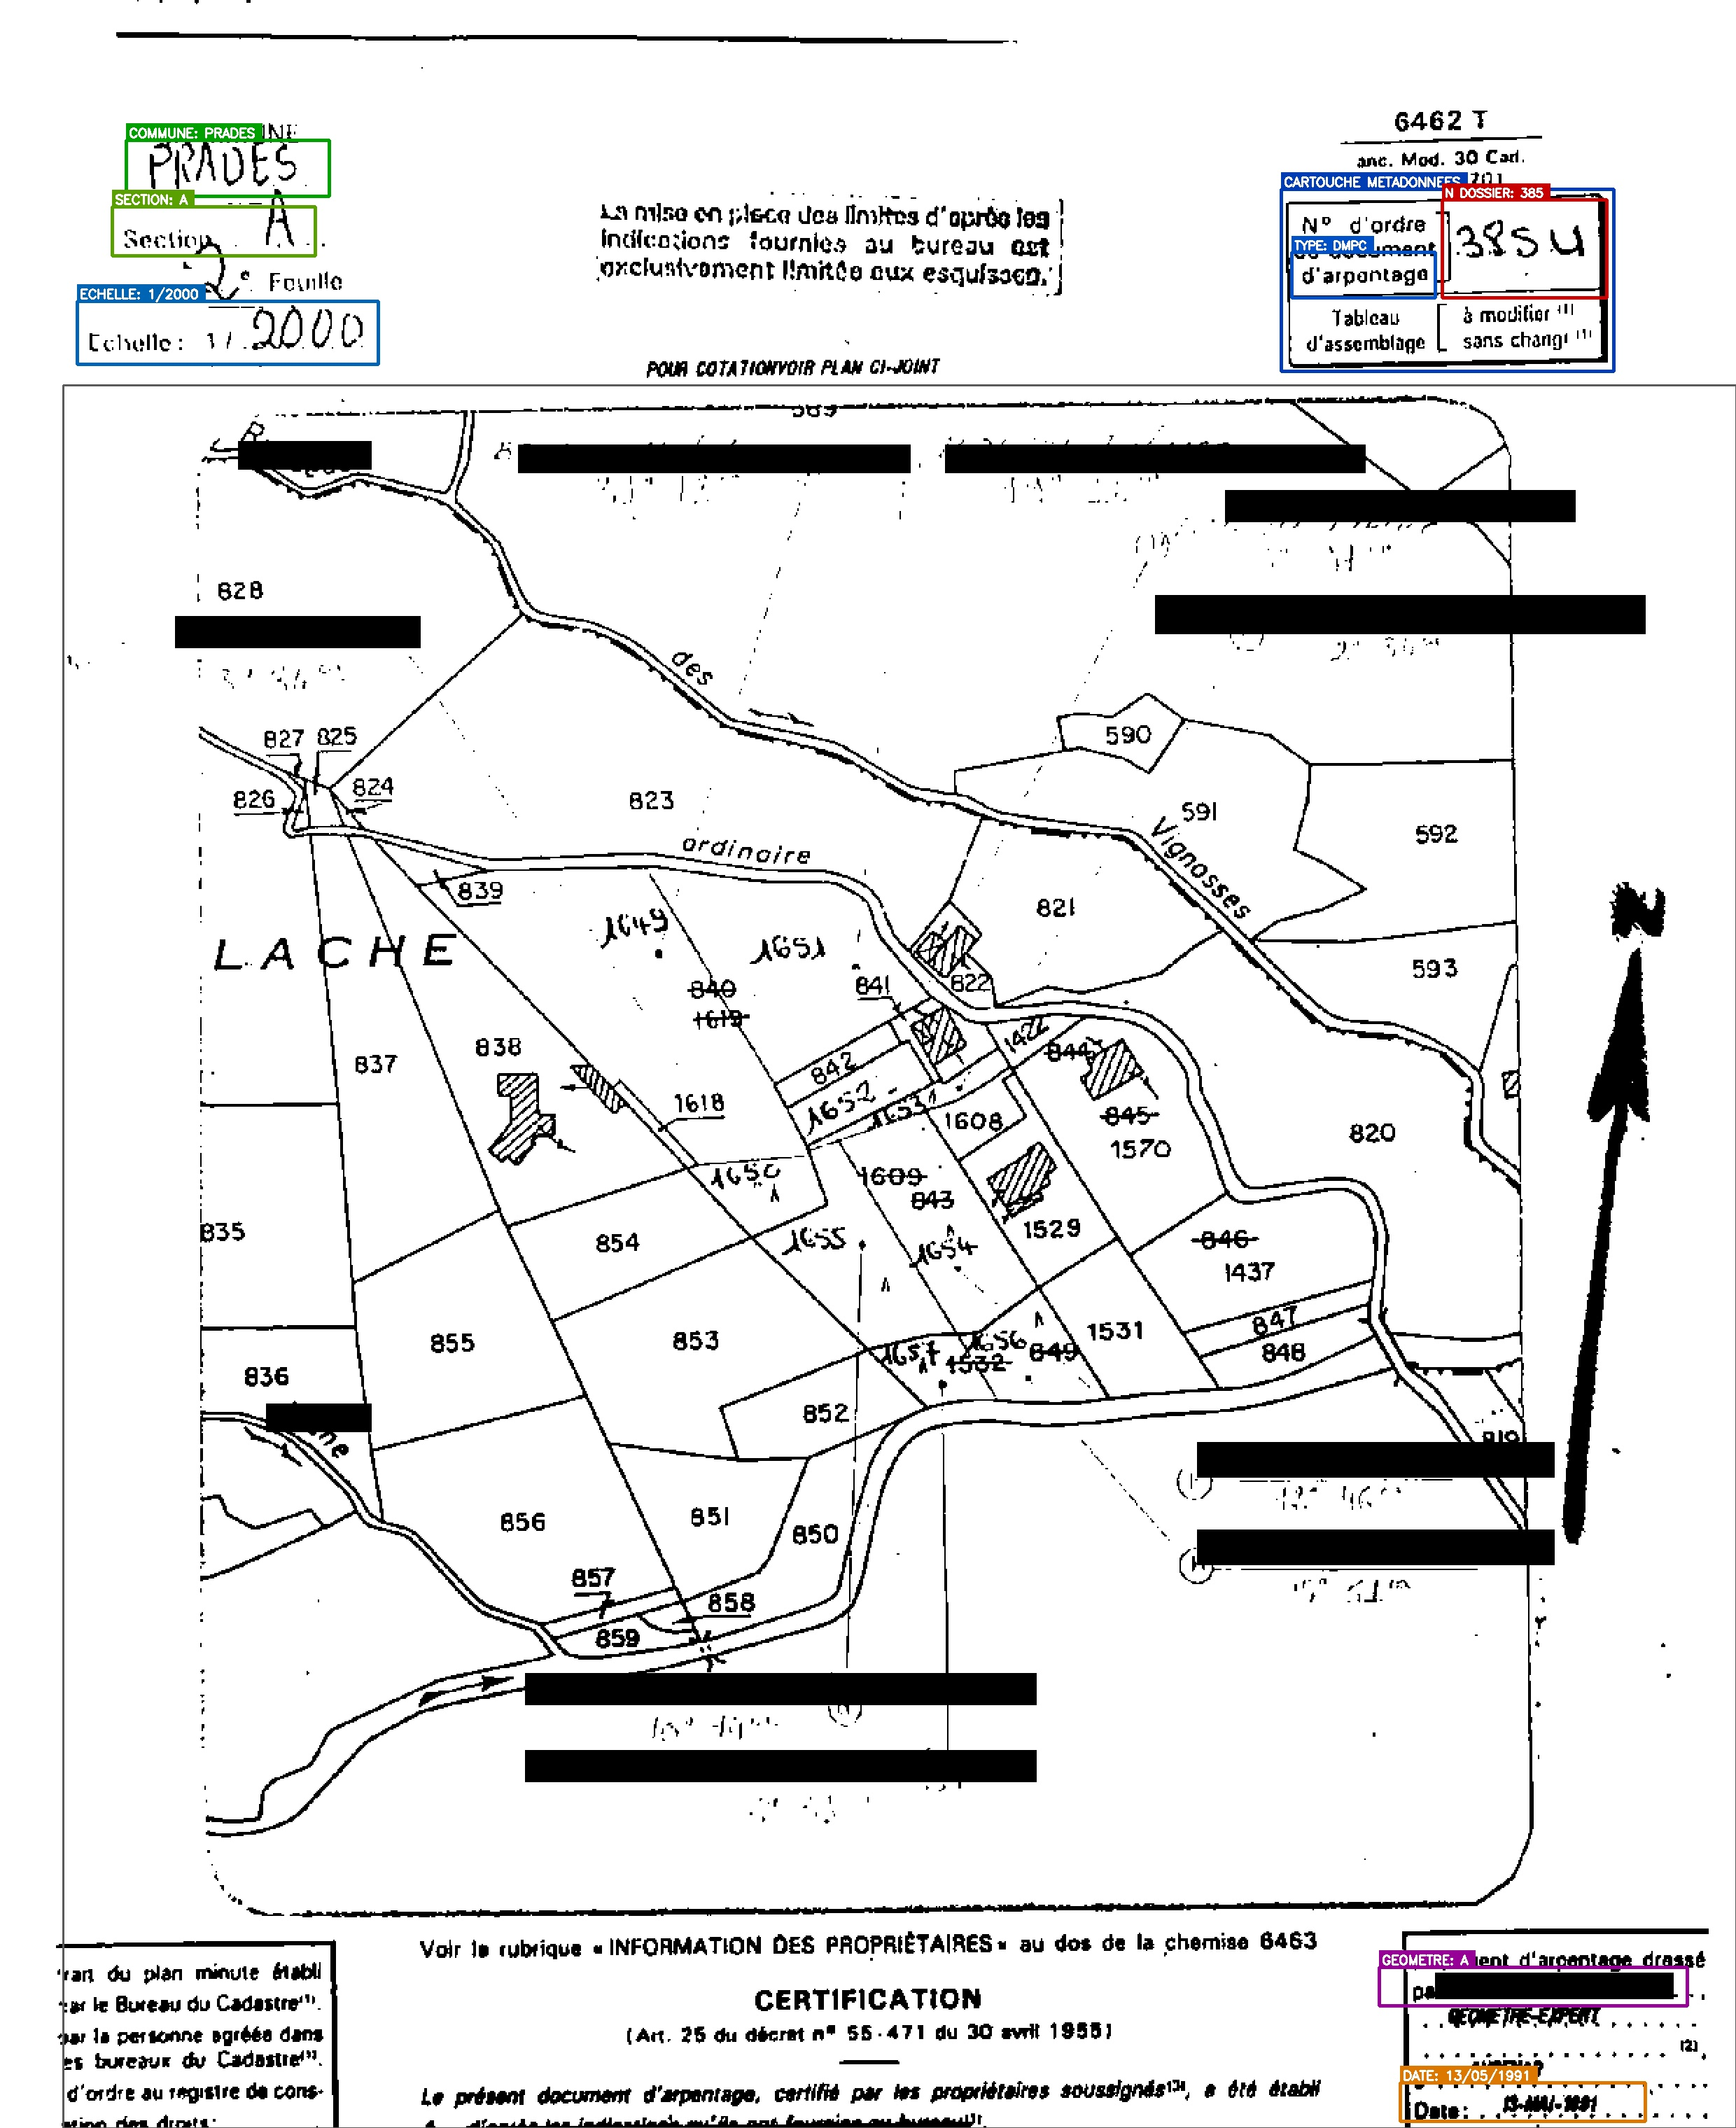
\includegraphics[width=0.85\textwidth]{img/harrois_annote.jpg}
  \caption{Image annotée du DMPC de Prades : les zones d'intérêt détectées par YOLOv8 sont encadrées sur le document source.}
  \label{fig:harrois_annote}
\end{figure}

L'interface de validation (présentée au chapitre~\ref{sec:fiabilisation}) affiche directement les données extraites du document. L'opérateur contrôle les informations, comme la commune ou la section, et corrige les petites erreurs si nécessaire, par exemple le numéro d'ordre (\texttt{3854} $\rightarrow$ \texttt{385}) perturbé par un tampon en marge.

À l'étape 1, la recherche dans le répertoire numérisé retrouve la référence interne du dossier au cabinet.

À l'étape 2, la carte interactive affiche la parcelle sur le fond cadastral IGN. L'opérateur vérifie qu'aucune pastille n'existe déjà à cet endroit, puis confirme la localisation. Les coordonnées GPS sont automatiquement converties en Lambert-93 par la fonction \texttt{latlon\_to\_lambert93()}.

À l'étape 3, l'interface affiche le récapitulatif complet des données avant l'envoi.

L'opérateur clique sur \enquote{Créer le dossier sur Géofoncier}. L'API retourne un code \texttt{201 Created} avec l'identifiant du dossier créé. Le fichier PDF est automatiquement joint au dossier dans la foulée. La confirmation s'affiche dans l'interface (Figure~\ref{fig:confirmation_geofoncier}).

\begin{figure}[H]
  \centering
  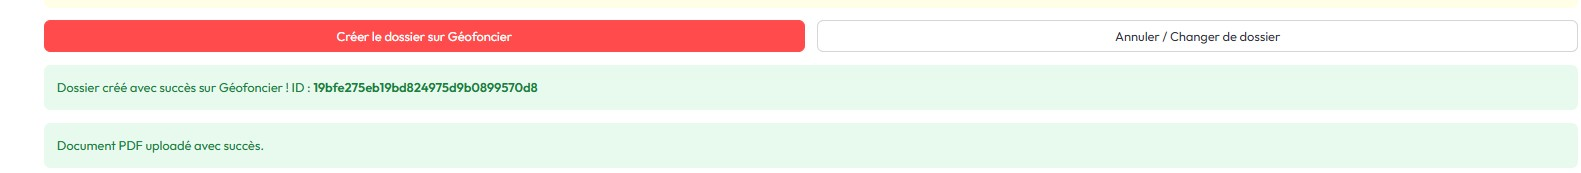
\includegraphics[width=0.95\textwidth]{img/6_succes_pastille.jpg}
  \caption{Confirmation de la création du dossier sur Géofoncier.}
  \label{fig:confirmation_geofoncier}
\end{figure}

Le dossier est désormais visible sur GéofoncierEXPERT sous forme de pastille géolocalisée, consultable par l'ensemble de la profession. Le statut de la ligne dans le fichier CSV local est automatiquement mis à jour avec la mention \texttt{Versé sur Géofoncier} et l'horodatage exact de la publication.

\subsection{Évaluation des performances}

Sans l'outil, retrouver un dossier dans les archives physiques prend au minimum une dizaine de minutes lorsque les boîtes sont bien organisées. Ce temps s'allonge si les dossiers sont mal rangés, si le registre du géomètre correspondant n'est pas encore numérisé, ou si plusieurs affaires correspondent aux mêmes références cadastrales.

Avec cet outil, le déroulement ne demande que quelques minutes de traitement OCR automatique (environ dix minutes pour un lot complet de cinq à six documents), suivies de deux ou trois minutes de contrôle dans l'interface pour relire les champs et valider la position cartographique, puis enfin quelques secondes pour le versement final par l'API.

Le temps d'intervention humaine est réduit à un contrôle de qualité sur des données déjà pré-remplies. La tâche n'est plus une recherche manuelle dans des archives physiques mais une validation d'un formulaire déjà instruit (chapitre~\ref{sec:fiabilisation}).

Le système a été testé sur une trentaine de documents couvrant plusieurs fonds et plusieurs types d'actes. Le Tableau~\ref{tab:qualite_extraction} présente une synthèse des observations par type de document.

\begin{table}[H]
  \centering
  \caption{Synthèse qualitative de l'extraction par type de document.}
  \label{tab:qualite_extraction}
  \small
  \begin{tabular}{p{3cm}p{3.5cm}p{3.5cm}p{2.5cm}}
    \toprule
    \textbf{Type} & \textbf{Champs fiables} & \textbf{Champs à vérifier} & \textbf{Score observé} \\
    \midrule
    DMPC imprimé récent & Commune, section, nature de l'acte & Numéro d'ordre (tampons), date & Souvent 100\,\% \\
    \addlinespace
    Document dactylographié & Commune (si lisible), section & Date, signataires, parcelles & 80--92\,\% \\
    \addlinespace
    Registre manuscrit & Commune, année, n° dossier & Noms de propriétaires, client & 78--85\,\% \\
    \addlinespace
    Croquis ou document libre & Commune, date (si présente) & Section, parcelles, référence & Variable \\
    \bottomrule
  \end{tabular}
\end{table}

Dans tous les cas, le contrôle humain reste obligatoire avant tout versement, et l'interface est conçue pour que cette vérification soit rapide. L'objectif du système n'est pas de supprimer l'intervention humaine, mais de réduire le temps qu'elle exige.

% A RELIRE
Pour compléter les observations qualitatives, une évaluation statistique des taux de réussite par champ a été réalisée sur le jeu de test. Les métriques mesurées (précision, rappel et score F1, dont la définition théorique a été donnée au chapitre~\ref{sec:etat_art}) sont récapitulées dans le Tableau~\ref{tab:precision_par_champ}.

\begin{table}[H]
  \centering
  \caption{Taux de précision et de rappel observés par champ d'indexation.}
  \label{tab:precision_par_champ}
  \small
  \begin{tabular}{p{4.5cm} c c c}
    \toprule
    \textbf{Champ d'indexation} & \textbf{Précision (\%)} & \textbf{Rappel (\%)} & \textbf{Score F1 (\%)} \\
    \midrule
    Nom de la commune & 97,0 & 94,1 & 95,5 \\
    Code INSEE & 97,0 & 97,0 & 97,0 \\
    Section cadastrale & 91,2 & 88,6 & 89,9 \\
    Numéro de parcelle & 88,5 & 85,0 & 86,7 \\
    Date de l'acte & 86,1 & 82,4 & 84,2 \\
    Nom du géomètre-expert & 94,1 & 91,3 & 92,7 \\
    Référence du dossier & 82,8 & 79,3 & 81,0 \\
    \bottomrule
  \end{tabular}
\end{table}

Les informations comme la commune et le code INSEE atteignent des taux de précision élevés grâce au découpage d'image par YOLOv8 (chapitre~\ref{sec:architecture}) et au filtrage géographique par la distance de Levenshtein (chapitre~\ref{sec:fiabilisation}). Les numéros de section et de parcelles atteignent un score F1 proche de 90\,\%, les erreurs résiduelles s'expliquant par la superposition de traits de dessin ou de pliures du papier. Enfin, les dates et références de dossiers extraites des registres affichent une précision de 81 à 84\,\%.
% >>>>>>>>>>>>>>>>>>>

Quelques situations posent des difficultés récurrentes. Les numéros de dossier interne sont rarement présents sur le plan lui-même et doivent être retrouvés dans les registres numérisés, ce qui n'est possible que pour les géomètres dont le répertoire a déjà été traité. Tant que certains fonds ne sont pas couverts, cette étape reste manuelle.

Par ailleurs, les parcelles très anciennes peuvent ne plus figurer dans la base cadastrale actuelle. La filiation parcellaire permet de remonter la chaîne dans la plupart des cas, mais certains historiques incomplets laissent des situations sans correspondance automatique.

Enfin, le temps de traitement par lot reste significatif sur un poste sans accélération GPU. Ce point, ainsi que les perspectives d'amélioration, sont abordés dans le chapitre suivant (chapitre~\ref{sec:limites_perspectives}).



